\section{Experiment 9D: uncertainty-triggered adaptive calibration}
\label{sec:experiment9d}

\paragraph{Question and staged protocol.}
Experiment 9D tests the implication of the 9C failure: if 0.25~s records are
structurally uninformative, can uncertainty trigger a small amount of targeted
additional excitation and recover useful label-free sharing? Seeds 126--135 are
used for development. The final acquisition policy and the unchanged hard gate
are then evaluated once on previously untouched seeds 136--145. Confirmation is
opened only after development passes.

Every client starts with three 0.25~s records at one locally assigned speed,
corresponding to 0.75~s total calibration. If the normalized Gauss--Newton
covariance trace exceeds 0.05, the client records a one-second maneuver at a
complementary speed and refits. At most two such follow-ups are permitted, so
the full fixed-budget comparator uses 2.75~s, still below the three-second 9B
baseline. The final policy was selected on development after a preliminary
variant with additional 0.25~s bursts showed that repeatedly restarting a very
short maneuver did not provide sufficient transient information. No
confirmation seed was accessed during that revision.

The proposed Adaptive-soft method applies the 9C heteroscedastic mixture and
posterior controller blending to each client's stopping-time estimate. It is
compared with Short-point, which applies ordinary learned-$K$ clustering to the
initial 0.75~s data; Fixed-full-soft, which always consumes 2.75~s; Local-
adaptive; Global-adaptive; and Oracle-adaptive, which uses simulated family
labels only for reference. The frozen gate requires Adaptive-soft to remain
within 5\% of Oracle-adaptive, strictly improve Short-point, use less mean data
than Fixed-full-soft, remain feasible and frozen-stable, and retain fewer shared
models than Local-adaptive.

\begin{table}[htbp]
\centering
\caption{Experiment 9D development and untouched-confirmation results.}
\label{tab:experiment9d-results}
\begin{tabular}{llrrrr}
\toprule
Phase & Method & Tracking & Models & Data [s] & Parameter error\\
\midrule
Development & Oracle-adaptive & 0.007610 & 3.0 & 1.75 & 0.0494\\
Development & Short-point & 0.012299 & 2.4 & 0.75 & 0.1791\\
Development & Adaptive-soft & 0.007886 & 2.9 & 1.75 & 0.0524\\
Development & Fixed-full-soft & 0.007594 & 3.0 & 2.75 & 0.0486\\
\midrule
Confirmation & Oracle-adaptive & 0.007542 & 3.0 & 1.75 & 0.0464\\
Confirmation & Short-point & 0.011666 & 2.7 & 0.75 & 0.1759\\
Confirmation & Adaptive-soft & 0.007758 & 2.8 & 1.75 & 0.0534\\
Confirmation & Fixed-full-soft & 0.007513 & 3.0 & 2.75 & 0.0451\\
\bottomrule
\end{tabular}
\end{table}

\begin{figure}[htbp]
\centering
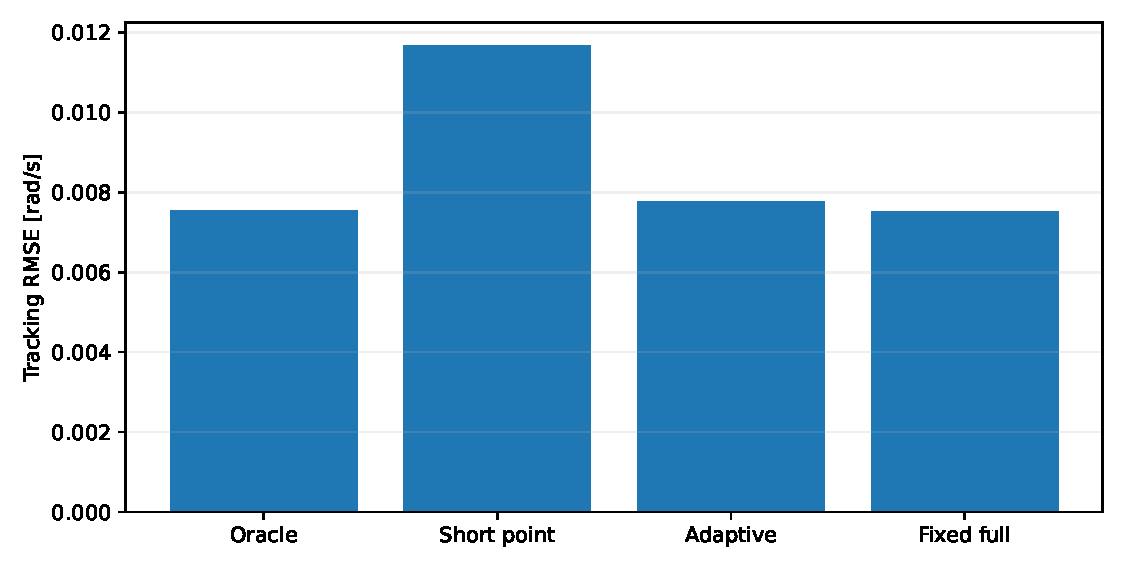
\includegraphics[width=0.78\linewidth]{../results/figures/experiment_9d_adaptive_calibration.pdf}
\caption{Untouched-confirmation tracking for the oracle, initial short-data,
adaptive, and fixed full-budget methods.}
\label{fig:experiment9d}
\end{figure}

\paragraph{Results.}
The development gate passes. Adaptive-soft is 3.62\% above Oracle-adaptive and
35.88\% better than Short-point. It selects 2.9 shared models on average,
achieves unseen hard-label ARI 0.935, and uses 1.75~s per client rather than the
2.75~s fixed full budget. Every client stops after the first one-second follow-
up, which means the covariance criterion gives a consistent stopping decision
in this benchmark rather than merely reducing the fleet-average budget.

The untouched confirmation gate also passes. Adaptive-soft tracking is
0.007758~rad/s, 2.86\% above Oracle-adaptive and 33.50\% better than Short-point.
It retains 2.8 shared models on average versus 30 Local-adaptive models, and
again stops at 1.75~s for every client. Confirmation hard-label ARI is lower,
0.820, yet soft membership preserves near-oracle control. This distinction is
important: exact recovery of simulator labels is neither necessary nor used by
the proposed control policy. Fixed-full-soft reaches 0.007513~rad/s, but needs
one additional second per client.

Across both stages, all 4,200 final client fits converge and all 10,800 nonlinear
closed-loop evaluations are amplitude-feasible. The worst frozen radius remains
below one. Local-adaptive still gives the lowest absolute tracking error
(0.006907~rad/s in confirmation), so the result is not an accuracy advantage
over a separate per-vehicle controller. Its contribution is a calibration--
deployment tradeoff: label-free sharing recovers near-oracle family performance
with 2.8 shared controllers and 1.75~s of local calibration.

\paragraph{Decision and FL interpretation.}
Experiment 9D resolves the short-data failure in the intended operational sense.
The federated system should not demand a fixed calibration budget from every
client or cluster estimates known to be uninformative. Instead, clients expose
compact estimates and uncertainty, the server learns shared compatibility
models, and uncertainty triggers additional local excitation only when needed.
This gives the paper a stronger control-specific FL message: federation changes
the data-acquisition decision as well as the estimator. Privacy is still absent
from group discovery and uncertainty reporting. A subsequent experiment may
combine this confirmed policy with the established private aggregation
mechanism, but should not alter the 9D acquisition rule.

\paragraph{Reproducibility.}
The frozen final protocol is in \path{code/config/experiment_9d.json}; the
implementation is in
\path{code/experiments/experiment_9d_adaptive_calibration.py}. Development and
confirmation seed summaries, budget statistics, group diagnostics, gate
decisions, and provenance hashes are retained under \path{results/tables}.
